%%%%%%%%
% Chapitre 6 %
%%%%%%%%

\chapter{La diffraction}
\section{Conditions de difraction}
	La plupart des méthodes modernes de la caractérisation de la structure et microstructure des solides sont basées sur la diffraction des ondes par les cristaux. Les longueurs d'ondes doivent être comparable à la distance entre les plans cristallins $\Rightarrow$ rayons X. La dualité onde corpuscule indique que le phénomène de diffraction peut se produire dans les solides cristallins. On a par exemple le microscope électronique qui permet de déterminer les réseaux cristallins et leur orientation. \\
	Soit une onde plane de longueur d'onde $\lambda$ se propageant dans une direction $\vec{n}$ de l'espace, on note
	\begin{equation}
		\psi (\vec{r},t)= A \exp \{i(2\pi \vec{k}\vec{r}-\omega t)\}\qquad \vec{k} = \frac{\vec{n}}{\lambda}
	\end{equation}
	où $k$ est le vecteur d'onde sans la convention où le $2\pi$ est compris dans $k$. Si $n$ est sans dimension, ce n'est pas le cas de sa norme qui s'exprime en $m^{-1}$. Pour simplifier, on considère une amplitude égal à 1 et on next la dépendance par rapport au temps pour avoir la distribution dans l'espace
	\begin{equation}
		\psi (\vec{r}) = \exp (2\pi i \vec{k}\vec{r})
	\end{equation}
	
	\subsection{Diffusion élastique d'une onde plane par un centre diffuseur ponctuel}
	\begin{wrapfigure}[8]{l}{5cm}
	\vspace{-5mm}
	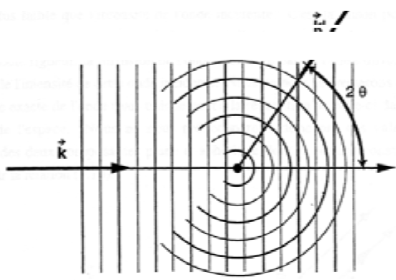
\includegraphics[scale=0.7]{ch6/1}
	\end{wrapfigure}
	La figure ci-contre représente la diffusion d'une onde plane par un centre diffuseur (un atome pour nous). La diffusion étant élastique donc sans perte d'énergie, les longueur d'onde sont égaux. Nous admettons que l'émission est cohérente, c'est à dire que l'onde incidente et l'onde diffusé sont en phase. L'amplitude de l'onde sphérique décroît avec la distance au centre. Considérons maintenant une direction n' faisant un angle $2\theta$ (convention) avec la direction n, menant à exprimer la fonction de l'onde en un point $r$ comme la somme de l'onde incidente et diffusée
	\begin{equation}
		\psi (\vec{r}) = \exp (2\pi i \vec{k}\vec{r}) + f(2\theta )\left(\frac{\exp (2\pi i \vec{k}'\vec{r})}{r} \right)
	\end{equation}
	où $f(2\theta )$ est le facteur de diffusion atomique qui dépend de la nature de l'onde plane et $\ll 1$. L'intensiré de l'onde diffusé est donc inférieur à l'intensité de l'onde incidente (justifiant l'amplitude de 1).   \newpage
	
	\subsection{Diffusion élastique d'une onde plane par deux atomes}
	\begin{wrapfigure}[5]{l}{5cm}
	\vspace{-5mm}
	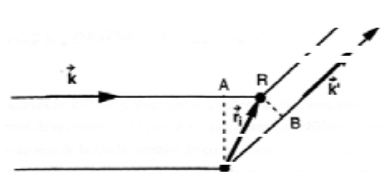
\includegraphics[scale=0.7]{ch6/2}
	\end{wrapfigure}
	Considérons à présent que deux atomes diffusent au lieu d'un seul. L'un est situé en $r=0$ et l'autre en $r=r_i$. Dans la direction $k'$ les ondes diffusées par chacune présentent une différence de marche $\delta = OB-AR=\lambda (\vec{k}'\vec{r}_i - \vec{k}\vec{r}_i)$ en se rappelant que la norme des fonctions vaut $\frac{1}{\lambda}$. La différence de phase s'exprime alors 
	\begin{equation}
		\frac{2\pi \delta}{\lambda} = 2\pi (\vec{k}'-\vec{k})\vec{r}
	\end{equation}
\section{Loi de Bragg}
\section{Applications}